\documentclass[11pt,a4paper]{article}

\usepackage[utf8]{inputenc}
\usepackage[margin=1in]{geometry}
\usepackage{xcolor}
\usepackage{graphicx}
\usepackage{hyperref}
\usepackage{booktabs}
\usepackage{tabularx}
\usepackage{enumitem}
\usepackage{fancyhdr}
\usepackage{tcolorbox}
\usepackage{titlesec}
\usepackage{float}
\usepackage{amssymb}

% Color Definitions (LevelUP Theme)
\definecolor{primaryOrange}{HTML}{EA580C}
\definecolor{darkObsidian}{HTML}{0B0C11}
\definecolor{lightCream}{HTML}{FBF7F4}
\definecolor{borderGray}{HTML}{E2D9CF}
\definecolor{accentEmerald}{HTML}{10B981}

\hypersetup{
    colorlinks=true,
    linkcolor=primaryOrange,
    urlcolor=primaryOrange,
    citecolor=primaryOrange
}

% Header and Footer Setup
\setlength{\headheight}{15pt}
\pagestyle{fancy}
\fancyhf{}
\fancyhead[L]{\textbf{\textcolor{primaryOrange}{LevelUP}} \textbar\ Project Solution Report}
\fancyhead[R]{\thepage}
\fancyfoot[C]{\footnotesize LevelUP Engineering Platform \textbar\ Competition Submission}
\renewcommand{\headrulewidth}{0.4pt}
\renewcommand{\footrulewidth}{0.4pt}

% Section Titles Styling
\titleformat{\section}{\Large\bfseries\color{primaryOrange}}{\thesection}{1em}{}[\titlerule]
\titleformat{\subsection}{\large\bfseries\color{darkObsidian}}{\thesubsection}{1em}{}
\titleformat{\subsubsection}{\normalsize\bfseries\color{primaryOrange}}{\thesubsubsection}{1em}{}

\tcbset{colback=lightCream,colframe=primaryOrange,fonttitle=\bfseries,coltitle=white,arc=3mm,boxrule=1pt}

\begin{document}

% ─── TITLE PAGE ─────────────────────────────────────────────────────────────
\begin{titlepage}
    \centering
    \vspace*{0.5cm}
    
    
\includegraphics[width=0.45\textwidth]{figures/brand_logo.png}\\[1.2cm]
    
    {\Huge \textbf{\textcolor{darkObsidian}{LevelUP: AI-Powered Career Operating System}}}\\[0.4cm]
    {\Large \textbf{\textcolor{primaryOrange}{Autonomous Multimodal Agent for Engineering Skill Mastery \& Task Scheduling}}}\\[1.0cm]
    
    \begin{tcolorbox}[colback=primaryOrange!5,colframe=primaryOrange,title=\textbf{Competition Submission Project Report}]
    \centering
    \textbf{Comprehensive Technical Architecture, Product Features \& Implementation Details}\\
    \textit{Powered by MiniMax-M3 LLM, Voice-First Tutoring, Vision Inspector, and 1-Click Kanban Auto-Scheduling}
    \end{tcolorbox}
    
    \vspace{1.2cm}
    
    \begin{minipage}{0.48\textwidth}
        \textbf{Primary GitHub Repository:}\\
        \href{https://github.com/Prajeeth-12/LevelUP-new}{github.com/Prajeeth-12/LevelUP-new}\\[0.3cm]
        \textbf{Secondary Remote:}\\
        \href{https://github.com/Prajeeth-12/LevelUP_HCL}{github.com/Prajeeth-12/LevelUP\_HCL}\\[0.3cm]
        \textbf{Branch:}\\
        \texttt{new-theme-layrs}
    \end{minipage}
    \hfill
    \begin{minipage}{0.48\textwidth}
        \textbf{Live Application URL:}\\
        \href{https://level-up-new.vercel.app}{level-up-new.vercel.app}\\[0.3cm]
        \textbf{Deployed Backend URL:}\\
        \href{https://levelup-new-backend.onrender.com}{levelup-new-backend.onrender.com}\\[0.3cm]
        \textbf{Submission Date:}\\
        August 29, 2026
    \end{minipage}
    
    \vfill
    {\small \textbf{Tech Stack:} FastAPI \textbar\ React 18 \textbar\ Tailwind CSS \textbar\ MiniMax-M3 LLM \textbar\ Firebase Firestore \textbar\ Web Speech API}
\end{titlepage}

\tableofcontents
\newpage

% ─── SECTION 1: EXECUTIVE SUMMARY ──────────────────────────────────────────
\section{Executive Summary \& Value Proposition}

\textbf{LevelUP} is an AI-powered personal career operating system and autonomous learning assistant built to solve the modern software engineering skill gap. Instead of overwhelming learners with static course catalogs or rigid checklists, LevelUP pairs each user with a proactive, multimodal AI mentor that dynamically benchmarks their skills against real-world job descriptions, schedules balanced Kanban sprints, and engages in voice-first 1-on-1 tutoring.

\subsection{The Problem: The Developer Learning Dilemma}
Modern software engineers face three critical bottlenecks:
\begin{enumerate}
    \item \textbf{Skill Overwhelm \& Fragmentation:} Roadmaps, tasks, interview prep, and code repositories live in disconnected silos.
    \item \textbf{Burnout \& Unrealistic Sprints:} Backlogs accumulate hundreds of tasks without consideration of realistic weekly cognitive bandwidth.
    \item \textbf{Passive Learning vs. Active Feedback:} Reading articles or watching videos produces an illusion of competence without hands-on architecture verification or conversational quizzing.
\end{enumerate}

\subsection{The LevelUP Solution}
LevelUP unifies career trajectory planning, daily execution, and active AI mentorship into a single cohesive operating system:
\begin{itemize}[leftmargin=1.5em]
    \item \textbf{1-Click Kanban Smart Auto-Scheduler:} Analyzes tasks across 3 boards and optimizes daily focus according to user-defined study hours (e.g., 12h/week).
    \item \textbf{Voice-First 1-on-1 AI Tutor:} Spoken conversational technical coaching, mock interview practice, and system design drills.
    \item \textbf{Multimodal Vision \& GitHub Inspector:} Deep analysis of architecture whiteboard drawings, system schemas, and live GitHub repositories.
    \item \textbf{Human-in-the-Loop Safety:} The AI proposes structured modifications as interactive \textit{Action Cards} requiring explicit human approval before touching database state.
\end{itemize}

\newpage

% ─── SECTION 2: AUTHENTICATION & ONBOARDING ────────────────────────────────
\section{Authentication \& Onboarding Experience}

LevelUP provides seamless, enterprise-grade authentication powered by Firebase Authentication with Google OAuth and Email/Password flows.

\begin{figure}[H]
    \centering
    \begin{minipage}{0.48\textwidth}
        \centering
        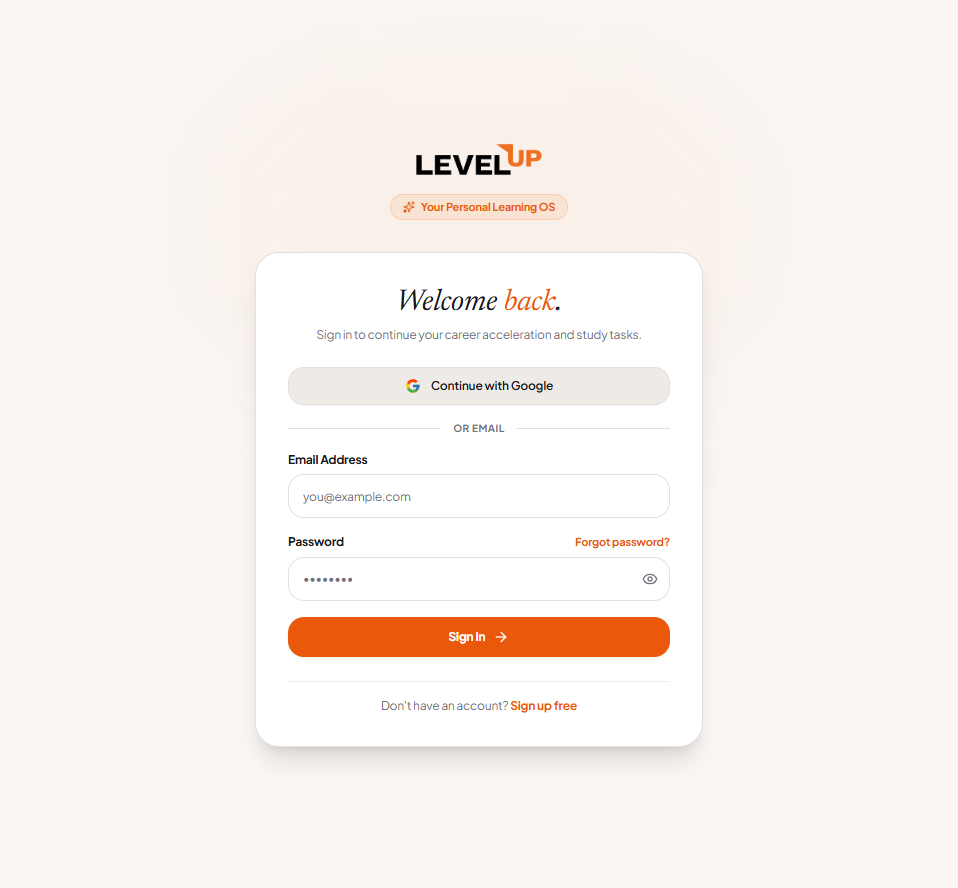
\includegraphics[width=\textwidth]{screenshots/01_signin.png}
        \caption{Sign In Page}
    \end{minipage}
    \hfill
    \begin{minipage}{0.48\textwidth}
        \centering
        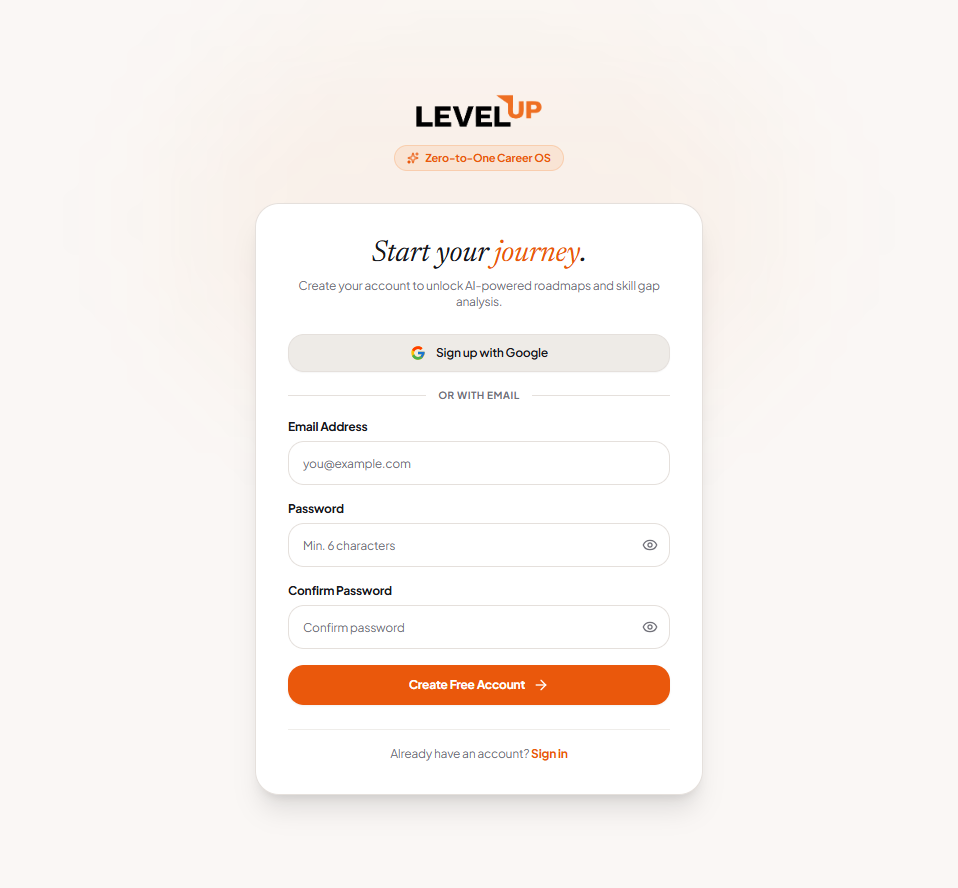
\includegraphics[width=\textwidth]{screenshots/02_signup.png}
        \caption{Sign Up / Create Account Page}
    \end{minipage}
\end{figure}

\subsection{Design Highlights}
\begin{itemize}[leftmargin=1.5em]
    \item \textbf{Warm Minimalist Layrs Theme:} Warm cream background with high-contrast typography, rounded-2xl cards, and orange accents.
    \item \textbf{Google One-Tap Authentication:} Instant onboarding with automatic profile initialization and token synchronization.
    \item \textbf{Inline Password Reset Flow:} Reset workflows embedded directly within the card context without disruptive page redirects.
\end{itemize}

\newpage

% ─── SECTION 3: CORE DASHBOARD & HOME BASE ─────────────────────────────────
\section{Core Dashboard \& Navigation Hub}

The LevelUP dashboard serves as the central mission control for the learner, integrating daily goals, active roadmaps, and cycle metrics in real time.

\begin{figure}[H]
    \centering
    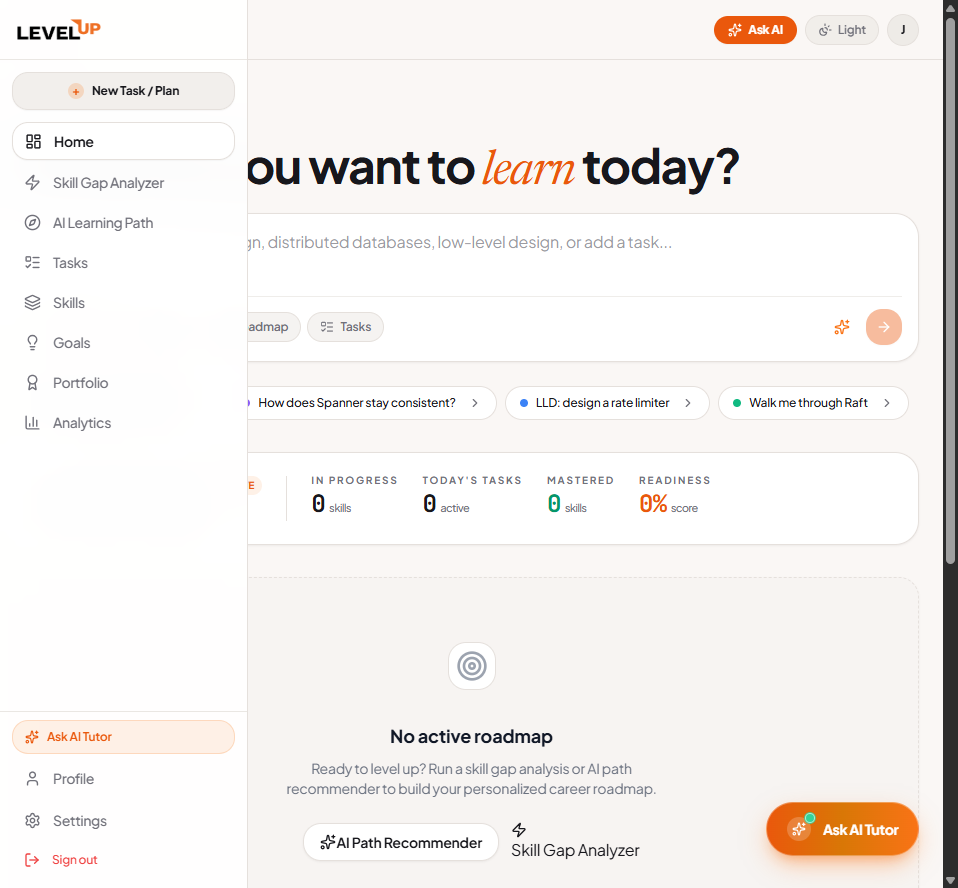
\includegraphics[width=0.92\textwidth]{screenshots/03_dashboard.png}
    \caption{LevelUP Core Dashboard with Daily Question Prompt, Cycle Stats, and Sidebar Navigation.}
\end{figure}

\subsection{Key Dashboard Modules}
\begin{itemize}[leftmargin=1.5em]
    \item \textbf{Daily Knowledge Prompt:} Interactive conversational input that connects directly to the AI Tutor.
    \item \textbf{Cycle Stats Bar:} Real-time counts of \textit{In Progress Skills}, \textit{Today's Tasks}, \textit{Mastered Skills}, and the aggregate \textit{Career Readiness Score}.
    \item \textbf{Active Roadmap Panel:} Quick overview of the current learning path (e.g., Full Stack \& AI Engineer) with quick action buttons.
    \item \textbf{Slim Rail Sidebar:} Collapsible navigation with static margin alignment that ensures page content never jumps or shifts during collapse.
\end{itemize}

\newpage

% ─── SECTION 4: SKILLS INVENTORY & MASTERY ─────────────────────────────────
\section{Skills Inventory \& Mastery Matrix}

The Skills module organizes developer competencies into hierarchical domains with progress percentages, target levels, and subskill breakdowns.

\begin{figure}[H]
    \centering
    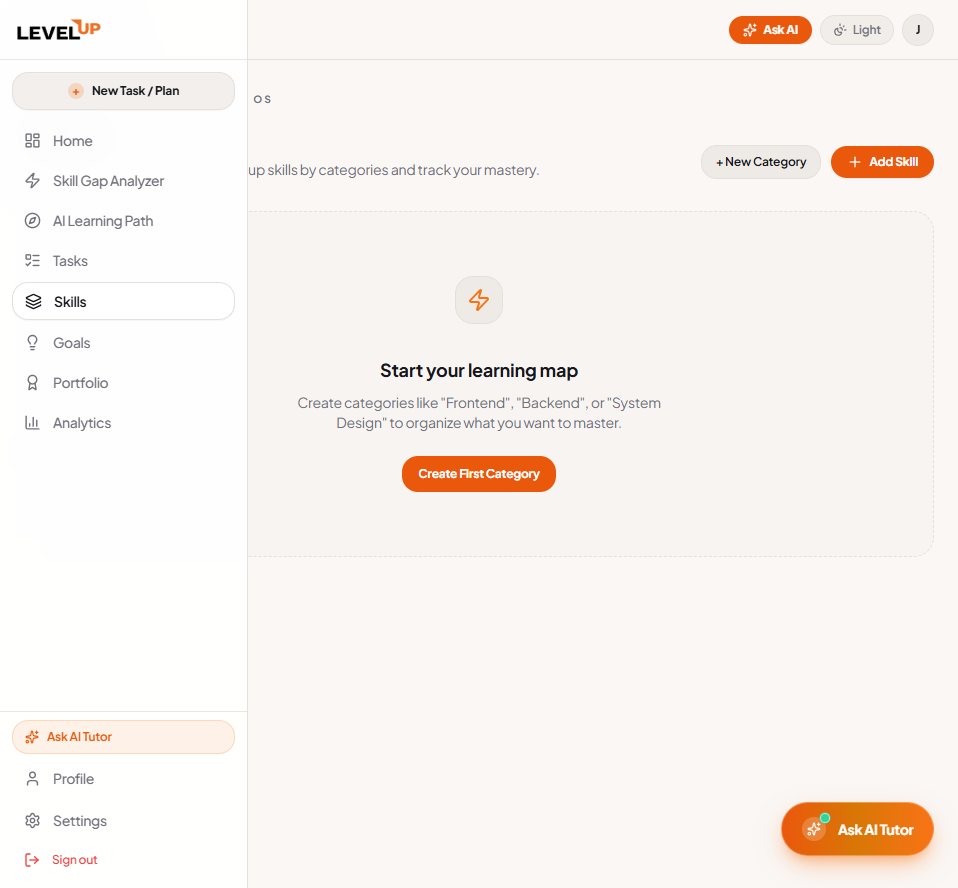
\includegraphics[width=0.92\textwidth]{screenshots/04_skills.png}
    \caption{Skills Board with Category Cards, Mastery Progress Indicators, and Priority Badges.}
\end{figure}

\subsection{Core Capabilities}
\begin{itemize}[leftmargin=1.5em]
    \item \textbf{Hierarchical Domain Categorization:} Skills organized by Frontend, Backend, Cloud/DevOps, System Design, and AI/ML.
    \item \textbf{Granular Subskill Breakdowns:} AI-generated subskills with completion checkboxes that automatically calculate parent skill mastery.
    \item \textbf{Readiness Score Impact:} Every progress increment dynamically updates the global career readiness algorithm on the home dashboard.
\end{itemize}

\newpage

% ─── SECTION 5: KANBAN BOARD & AUTO-SCHEDULER ──────────────────────────────
\section{3-Column Kanban Board \& 1-Click AI Auto-Scheduler}

The Tasks board implements a focused 3-column Kanban workflow: \textbf{To Do}, \textbf{Current (In Progress)}, and \textbf{Past (Completed)}.

\begin{figure}[H]
    \centering
    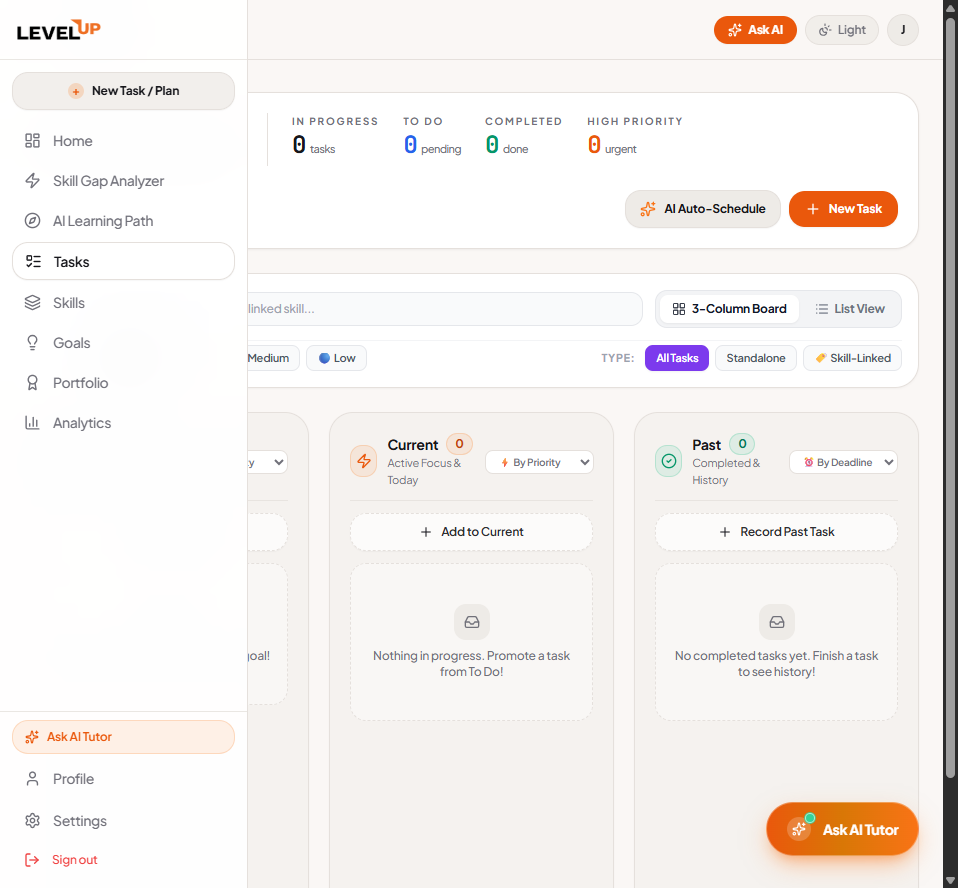
\includegraphics[width=0.92\textwidth]{screenshots/05_tasks.png}
    \caption{Tasks Board with 3-Column Kanban Layout and the AI Auto-Schedule System.}
\end{figure}

\subsection{The 1-Click AI Auto-Schedule Engine}
When the learner clicks \textbf{"AI Auto-Schedule"}, the system:
\begin{enumerate}[leftmargin=1.5em]
    \item Reads all active tasks and checks the user's weekly study budget (e.g., 12 hours/week).
    \item Analyzes deadlines, priorities, and cognitive complexity.
    \item Selects 2--4 high-leverage tasks for today's active sprint (~2--4 hours).
    \item Generates a pedagogical rationale explaining why this schedule maximizes learning velocity while preventing burnout.
    \item Renders an interactive modal allowing the user to review and selectively approve the proposed moves.
\end{enumerate}

\newpage

% ─── SECTION 6: SKILL GAP ANALYZER ─────────────────────────────────────────
\section{Skill Gap Analyzer \& AI Path Generator}

The Skill Gap Analyzer benchmarks a learner's existing skills against target engineering job descriptions.

\begin{figure}[H]
    \centering
    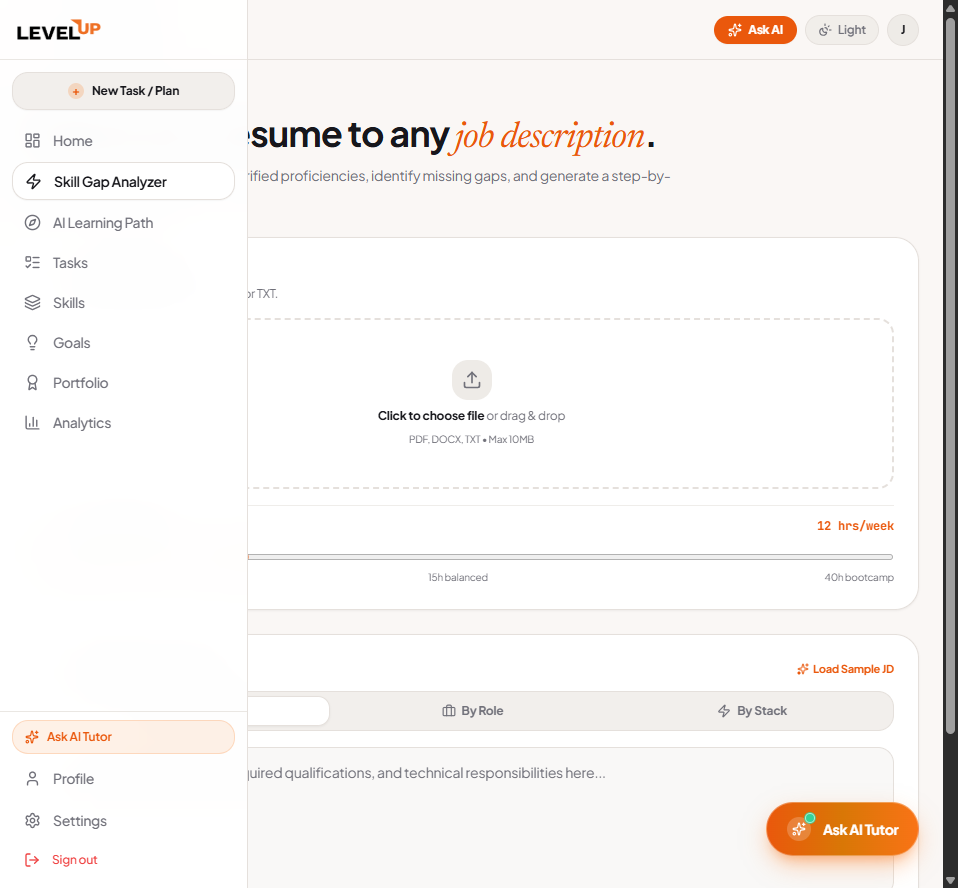
\includegraphics[width=0.92\textwidth]{screenshots/06_skillgap.png}
    \caption{Skill Gap Analyzer with Role Presets, Custom Job Description Input, and Phase Roadmap.}
\end{figure}

\subsection{Workflow \& Intelligence}
\begin{itemize}[leftmargin=1.5em]
    \item \textbf{Target Role Presets:} Pre-configured industry benchmarks for Full Stack, Backend, Frontend, DevOps, and AI Engineer roles.
    \item \textbf{Custom JD Extraction:} Pasting any job posting triggers MiniMax LLM extraction of required competencies vs. missing gaps.
    \item \textbf{Actionable Roadmap Generation:} Creates a chronological, phased learning roadmap with curated resources and estimated completion hours.
\end{itemize}

\newpage

% ─── SECTION 7: LEARNING ANALYTICS & GOALS ─────────────────────────────────
\section{Learning Analytics, Metrics \& Goal Tracking}

LevelUP provides deep visibility into study habits, task velocity, and skill acquisition over time.

\begin{figure}[H]
    \centering
    \begin{minipage}{0.48\textwidth}
        \centering
        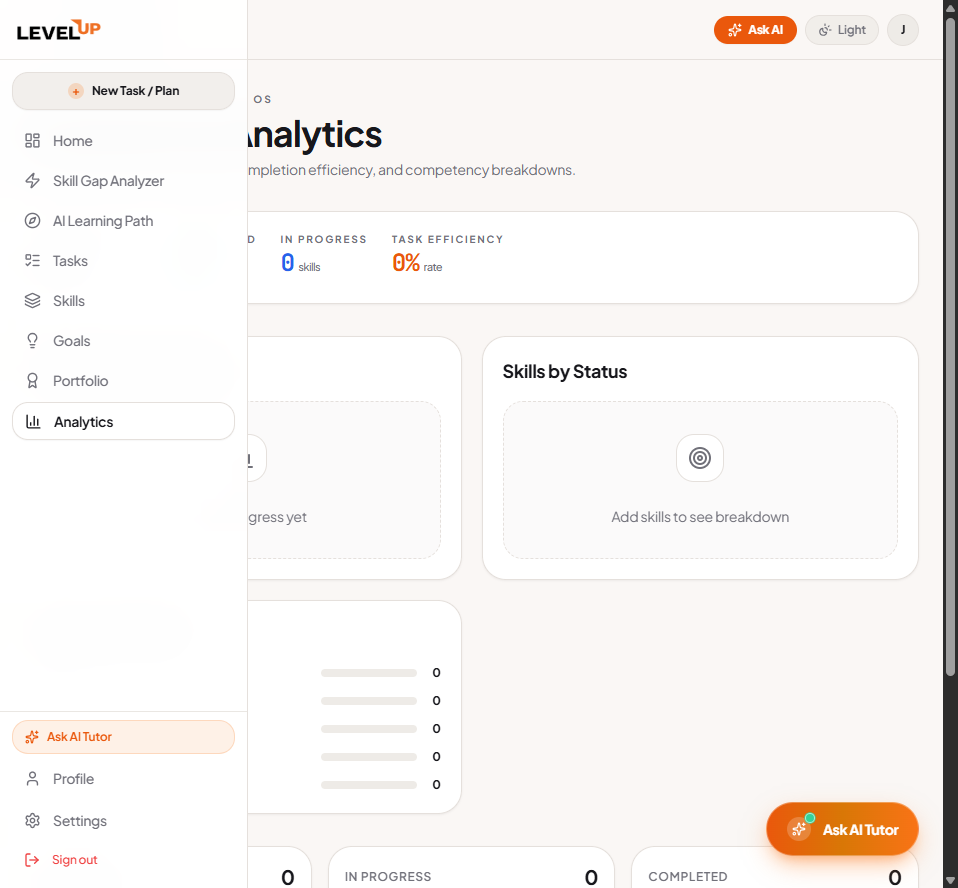
\includegraphics[width=\textwidth]{screenshots/07_analytics.png}
        \caption{Analytics \& Progress Insights}
    \end{minipage}
    \hfill
    \begin{minipage}{0.48\textwidth}
        \centering
        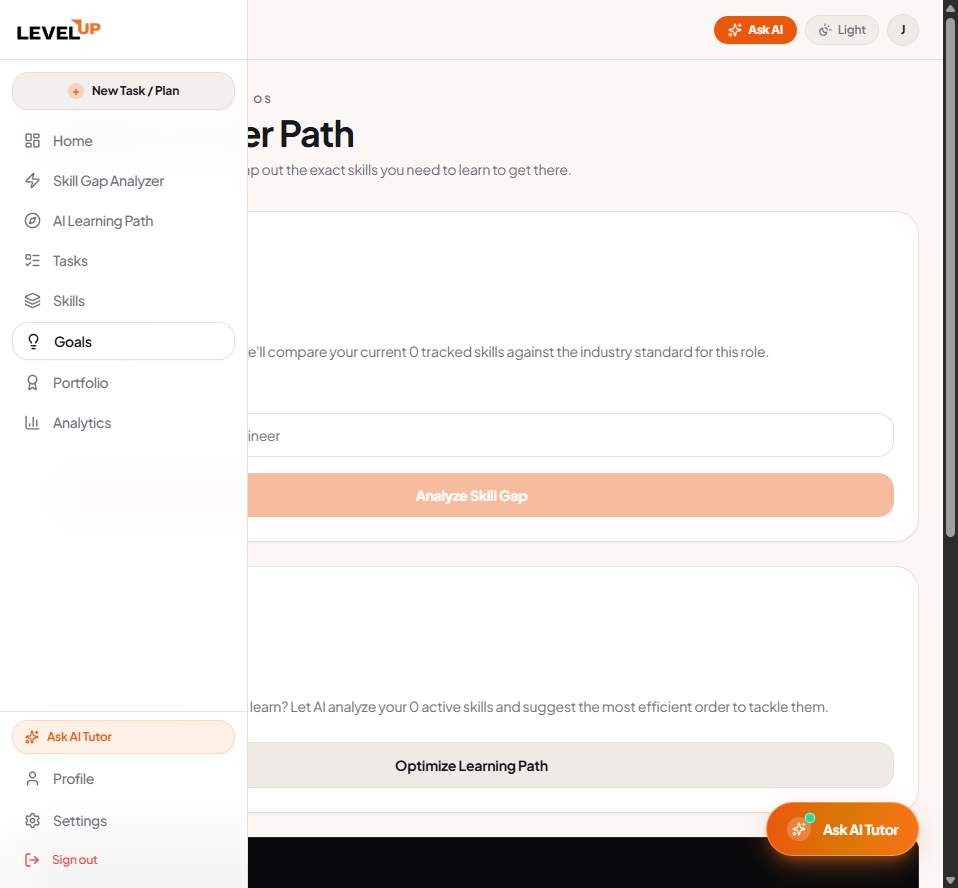
\includegraphics[width=\textwidth]{screenshots/09_goals.png}
        \caption{Goals \& Milestones Tracker}
    \end{minipage}
\end{figure}

\subsection{Analytics \& Insights Features}
\begin{itemize}[leftmargin=1.5em]
    \item \textbf{Mastery Distribution Charts:} Visual breakdown of skill progress across core domains.
    \item \textbf{Study Cadence Heatmaps:} Track daily task completion and identify consistency streaks.
    \item \textbf{Milestone Tracking:} Target completion dates aligned with career roadmaps and readiness targets.
\end{itemize}

\newpage

% ─── SECTION 8: AI MULTIMODAL CAPABILITIES ─────────────────────────────────
\section{AI Multimodal Capabilities \& Superpowers}

\subsection{1. MiniMax-M3 LLM Integration}
The platform utilizes the high-context MiniMax-M3 LLM (via OpenAI-compatible API) for deep engineering reasoning:
\begin{itemize}[leftmargin=1.5em]
    \item \textbf{Live Context Injection:} System prompt automatically includes the user's active skills, tasks, and roadmaps.
    \item \textbf{Structured JSON Output:} Responses return structured Markdown plus optional action payloads for automated workspace updates.
\end{itemize}

\subsection{2. Voice-First 1-on-1 AI Tutor}
\begin{itemize}[leftmargin=1.5em]
    \item \textbf{Speech-to-Text:} Web Speech API integration with animated mic waveform in the chat drawer.
    \item \textbf{Text-to-Speech:} Natural voice audio playback of technical answers with instant stop control.
    \item \textbf{Lifecycle Safety:} Speech and recognition sessions automatically terminate when closing the drawer or unmounting.
\end{itemize}

\subsection{3. Multimodal Vision \& GitHub Inspector}
\begin{itemize}[leftmargin=1.5em]
    \item \textbf{Diagram Analysis:} Drag-and-drop architecture sketches or database ERDs directly into chat.
    \item \textbf{GitHub Repository Inspection:} Paste repository URLs to automatically analyze project structure, languages, and patterns.
\end{itemize}

\subsection{4. Human-in-the-Loop Workspace Actions}
All AI-suggested changes (adding tasks, creating skills, updating progress) render as interactive \textit{Action Cards} with \texttt{[+ Approve \& Save]} buttons, guaranteeing human oversight.

\newpage

% ─── SECTION 9: TECHNICAL ARCHITECTURE & API REFERENCE ─────────────────────
\section{Technical Architecture \& API Reference}

\subsection{System Architecture Matrix}

\begin{table}[H]
\centering
\small
\begin{tabularx}{\textwidth}{l p{3.8cm} X}
\toprule
\textbf{Component} & \textbf{Technology} & \textbf{Description} \\
\midrule
\textbf{Frontend} & React 18, Vite, Tailwind CSS & Single-page application with responsive Layrs theme, adaptive sidebar, and rich Markdown rendering. \\
\addlinespace
\textbf{Backend} & FastAPI, Python 3.10+, Uvicorn & Asynchronous REST API, CORS middleware, and LLM prompt orchestration. \\
\addlinespace
\textbf{AI Engine} & MiniMax-M3 LLM & Advanced reasoning engine for roadmap synthesis, task scheduling, and vision analysis. \\
\addlinespace
\textbf{Database} & Google Cloud Firestore & Real-time NoSQL document store with reactive client snapshot listeners. \\
\addlinespace
\textbf{Auth} & Firebase Authentication & JWT token verification, Google OAuth, and secure guest access. \\
\bottomrule
\end{tabularx}
\caption{LevelUP Full-Stack Architecture Matrix}
\end{table}

\subsection{Core API Endpoints}

\begin{table}[H]
\centering
\small
\begin{tabularx}{\textwidth}{l l X}
\toprule
\textbf{Method} & \textbf{Endpoint} & \textbf{Functionality} \\
\midrule
\texttt{POST} & \texttt{/ai/chat} & Process chat messages with context, image inspection, and action generation. \\
\texttt{POST} & \texttt{/ai/auto-organize-tasks} & 1-Click Kanban sprint scheduler based on weekly hour budget. \\
\texttt{POST} & \texttt{/ai/skill-gap} & Extract missing skills and generate learning paths from role/JD. \\
\texttt{POST} & \texttt{/ai/generate-subskills} & Decompose a skill into actionable subskills. \\
\texttt{POST} & \texttt{/ai/task-plan} & Prioritize and order tasks based on available study time. \\
\texttt{POST} & \texttt{/ai/progress-insights} & Generate coaching recommendations based on activity history. \\
\texttt{POST} & \texttt{/api/students/profile} & Create and update student career profiles in Firestore. \\
\texttt{GET}  & \texttt{/api/career/roadmap} & Fetch active personalized career roadmap for a user. \\
\bottomrule
\end{tabularx}
\caption{Core Backend API Route Summary}
\end{table}

\newpage

% ─── SECTION 10: LOCAL SETUP & DEPLOYMENT GUIDE ────────────────────────────
\section{Local Setup \& Execution Guide}

\subsection{Step 1: Backend Setup (FastAPI)}
\begin{enumerate}[leftmargin=1.5em]
    \item Navigate to the backend directory: \texttt{cd backend}
    \item Create and activate a virtual environment:
    \begin{itemize}
        \item Windows: \texttt{python -m venv venv} \textbar\ \texttt{.\\venv\\Scripts\\activate}
        \item macOS/Linux: \texttt{python3 -m venv venv} \textbar\ \texttt{source venv/bin/activate}
    \end{itemize}
    \item Install dependencies: \texttt{pip install -r requirements.txt}
    \item Configure \texttt{backend/.env}:
    \begin{itemize}
        \item \texttt{MINIMAX\_API\_KEY=<your-key>}
        \item \texttt{MINIMAX\_BASE\_URL=https://api.gmi-serving.com/v1}
        \item \texttt{MINIMAX\_MODEL=MiniMaxAI/MiniMax-M3}
    \end{itemize}
    \item Start the backend: \texttt{python -m uvicorn app.main:app --port 8000 --reload}
\end{enumerate}

\subsection{Step 2: Frontend Setup (React + Vite)}
\begin{enumerate}[leftmargin=1.5em]
    \item Navigate to frontend directory: \texttt{cd frontend}
    \item Install dependencies: \texttt{npm install}
    \item Start development server: \texttt{npm run dev}
    \item Open in browser: \href{http://localhost:3000}{http://localhost:3000}
\end{enumerate}

\subsection{Step 3: Production Deployment Verification}
\begin{itemize}[leftmargin=1.5em]
    \item \textbf{Frontend (Vercel):} \href{https://level-up-new.vercel.app}{https://level-up-new.vercel.app}
    \item \textbf{Backend (Render):} \href{https://levelup-new-backend.onrender.com}{https://levelup-new-backend.onrender.com}
    \item \textbf{GitHub Repository:} \href{https://github.com/Prajeeth-12/LevelUP-new}{https://github.com/Prajeeth-12/LevelUP-new} (Branch: \texttt{new-theme-layrs})
\end{itemize}

\end{document}
